% Schematic of the ensemble SNN (E-SNN) and the spike-input control (Enc-ANN).
% Build: tectonic paper/figures/fig_architecture.tex   (or: python scripts/make_figures.py)
% Intended width: full text width of an IEEE two-column paper (7.16 in).
\documentclass[border=1pt]{standalone}
\usepackage[T1]{fontenc}
\usepackage{newtxtext,newtxmath}
\usepackage{tikz}
\usetikzlibrary{positioning,arrows.meta,fit,backgrounds,calc}

% Okabe-Ito colours (colourblind safe); fills are light so text stays legible in grayscale.
\definecolor{oiblue}{HTML}{0072B2}
\definecolor{oiorange}{HTML}{E69F00}
\definecolor{oigreen}{HTML}{009E73}
\definecolor{oiverm}{HTML}{D55E00}
\definecolor{oigray}{HTML}{555555}

\begin{document}
\fontsize{8}{9.4}\selectfont
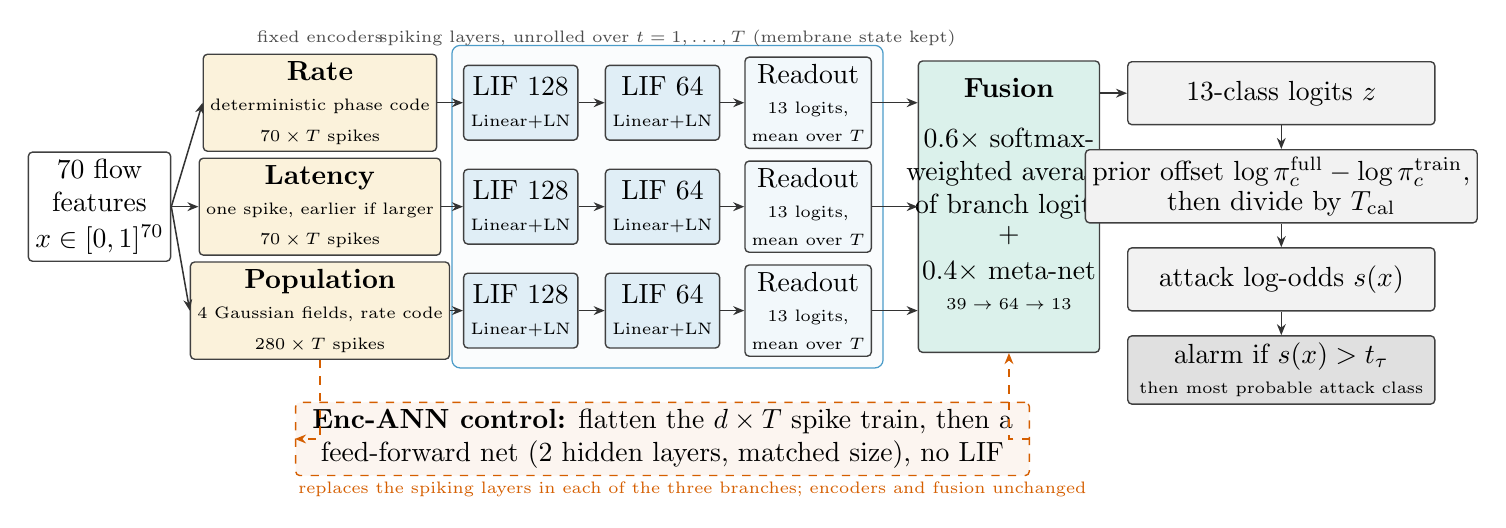
\begin{tikzpicture}[
  >={Stealth[length=4pt,width=3.2pt]},
  box/.style={draw=black!75, rounded corners=1.5pt, line width=0.5pt, align=center,
              inner sep=2.5pt, minimum height=0.95cm},
  enc/.style={box, fill=oiorange!14, minimum width=2.75cm, minimum height=1.05cm},
  lif/.style={box, fill=oiblue!12, minimum width=1.45cm},
  rd/.style={box, fill=oiblue!5, minimum width=1.6cm},
  fus/.style={box, fill=oigreen!14},
  dec/.style={box, fill=black!5, minimum width=3.9cm, minimum height=0.8cm},
  ctl/.style={box, inner xsep=6pt, dashed, draw=oiverm, fill=oiverm!6, text=black},
  flow/.style={->, line width=0.55pt, draw=black!80},
  cflow/.style={->, line width=0.6pt, dashed, draw=oiverm},
  dim/.style={font=\fontsize{6.5}{7.5}\selectfont, text=black!70, inner sep=1pt},
]

% ---------------- input ----------------
\node[box, fill=white, minimum width=1.55cm, minimum height=1.35cm] (in) at (0,0)
  {70 flow\\features\\[1pt] $x\in[0,1]^{70}$};

% ---------------- encoders (fixed, no parameters) ----------------
\def\ys{1.32}
\node[enc] (e1) at (2.8, \ys) {\textbf{Rate}\\[-1pt]{\fontsize{6.5}{7.5}\selectfont deterministic phase code}\\[-1pt]{\fontsize{6.5}{7.5}\selectfont $70\times T$ spikes}};
\node[enc] (e2) at (2.8, 0)   {\textbf{Latency}\\[-1pt]{\fontsize{6.5}{7.5}\selectfont one spike, earlier if larger}\\[-1pt]{\fontsize{6.5}{7.5}\selectfont $70\times T$ spikes}};
\node[enc] (e3) at (2.8,-\ys) {\textbf{Population}\\[-1pt]{\fontsize{6.5}{7.5}\selectfont 4 Gaussian fields, rate code}\\[-1pt]{\fontsize{6.5}{7.5}\selectfont $280\times T$ spikes}};
\coordinate (lab) at (0,2.08);
\node[dim, anchor=base] at (2.8,2.08) {fixed encoders};

\foreach \e in {e1,e2,e3} \draw[flow] (in.east) -- (\e.west);

% ---------------- spiking branches ----------------
\foreach \i/\y in {1/\ys, 2/0, 3/-\ys} {
  \node[lif] (a\i) at (5.35,\y) {LIF 128\\[-1pt]{\fontsize{6.5}{7.5}\selectfont Linear+LN}};
  \node[lif] (b\i) at (7.15,\y) {LIF 64\\[-1pt]{\fontsize{6.5}{7.5}\selectfont Linear+LN}};
  \node[rd]  (r\i) at (9.0,\y) {Readout\\[-1pt]{\fontsize{6.5}{7.5}\selectfont 13 logits,}\\[-2pt]{\fontsize{6.5}{7.5}\selectfont mean over $T$}};
  \draw[flow] (e\i.east) -- (a\i.west);
  \draw[flow] (a\i.east) -- (b\i.west);
  \draw[flow] (b\i.east) -- (r\i.west);
}
\begin{scope}[on background layer]
  \node[draw=oiblue!70, rounded corners=3pt, line width=0.45pt, fill=oiblue!2,
        fit=(a1)(b3)(r1)(r3), inner xsep=4pt, inner ysep=4pt] (snnbox) {};
\end{scope}
\node[dim, anchor=base] at (snnbox.north |- lab) {%
  spiking layers, unrolled over $t=1,\dots,T$ (membrane state kept)};

% ---------------- fusion ----------------
\node[fus, minimum width=2.3cm, minimum height=3.7cm] (fu) at (11.55,0) {};
\node[align=center, anchor=north] at ($(fu.north)+(0,-3pt)$) {\textbf{Fusion}};
\node[align=center] at ($(fu.center)+(0,0.42)$) {$0.6\times$ softmax-\\weighted average\\of branch logits};
\node at ($(fu.center)+(0,-0.37)$) {$+$};
\node[align=center] at ($(fu.center)+(0,-1.0)$) {$0.4\times$ meta-net\\[-1pt]{\fontsize{6.5}{7.5}\selectfont $39\to64\to13$}};
\foreach \i in {1,2,3} \draw[flow] (r\i.east) -- (r\i.east -| fu.west);

% ---------------- decision rule ----------------
\node[dec, anchor=north west] (lg) at (13.05, 1.85) {13-class logits $z$};
\node[dec, below=0.30cm of lg] (cal)
  {prior offset $\log\pi^{\mathrm{full}}_c-\log\pi^{\mathrm{train}}_c$,\\[-1pt]then divide by $T_{\mathrm{cal}}$};
\node[dec, below=0.30cm of cal] (s) {attack log-odds $s(x)$};
\node[dec, below=0.30cm of s, fill=black!12] (th)
  {alarm if $s(x)>t_\tau$\\[-1pt]{\fontsize{6.5}{7.5}\selectfont then most probable attack class}};
\draw[flow] (fu.east |- lg.west) -- (lg.west);
\draw[flow] (lg) -- (cal);
\draw[flow] (cal) -- (s);
\draw[flow] (s) -- (th);

% ---------------- spike-input control (Enc-ANN) ----------------
\node[ctl, minimum width=6.4cm, minimum height=0.8cm, anchor=center] (ctl) at (7.15,-2.95)
  {\textbf{Enc-ANN control:} flatten the $d\times T$ spike train, then a\\
   feed-forward net (2 hidden layers, matched size), no LIF};
\draw[cflow] (e3.south) |- (ctl.west);
\draw[cflow] (ctl.east) -| (fu.south);
\node[dim, text=oiverm, anchor=north west] at ($(ctl.south west)+(0,-1pt)$)
  {replaces the spiking layers in each of the three branches; encoders and fusion unchanged};

\end{tikzpicture}
\end{document}
